\section{Problem Description}\label{sec:problem_description}
By considering a free body diagram for the helicopter, such as the one in figure \ref{fig:heli_head_free_body} and figure \ref{fig:heli_body_free_body}, we can derive the equations of motion as seen in equation \ref{eq:model}. Here, we assume an already implemented PID controller for the elevation, as well as an already implemented PD controller for the pitch. This leaves only the open loop travel. An explanation of the symbols used are given in table \ref{tab:model_variables}.
\begin{subequations}\label{eq:model}
	\begin{gather}
		\ddot{e} + K_{3} K_{ed} \dot{e} + K_{3} K_{ep} e = K_{3} K_{ep} e_{c}\\
		\ddot{p} + K_{1} K_{pd} \dot{p} + K_{1} K_{pp} p = K_{1} K_{pp} p_{c}\\
		\dot{\lambda} = r\\
		\dot{r} = -K_{2} p
	\end{gather}
\end{subequations}
\begin{figure}[hb]
    \centering
    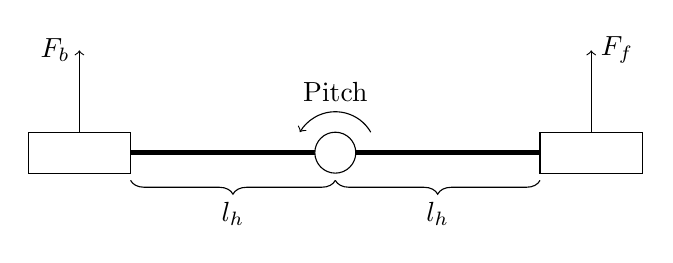
\begin{tikzpicture}[scale=1.3]
\usetikzlibrary{decorations.pathreplacing}
% Body
\path[draw,ultra thick] (1,1) -- ++(5,0);
\path[draw,fill=white] (3,1) circle (0.2);
\path[draw,fill=white] (0,0.8) rectangle ++(1,0.4);
\path[draw,fill=white] (5,0.8) rectangle ++(1,0.4);
% Forces and labels
\path[draw,->] (3,1) ++ (30:0.4) arc (30:150:0.4) node[midway, above] {Pitch};
\path[draw,->] (0.5,1.2) -- ++(0,0.8) node[left] {$F_b$};
\path[draw,->] (5.5,1.2) -- ++(0,0.8) node[right] {$F_f$};
\draw[decorate,decoration={brace,amplitude=5pt,raise=10pt,mirror}] (1,1) -- (3,1)
node[midway,below=0.5cm] {$l_h$};
\draw[decorate,decoration={brace,amplitude=5pt,raise=10pt,mirror}] (3,1) -- (5,1)
node[midway,below=0.5cm] {$l_h$};
\end{tikzpicture}
    \caption{Helicopter head free body diagram.}
    \label{fig:heli_head_free_body}
\end{figure}
\begin{figure}[hb]
    \centering
    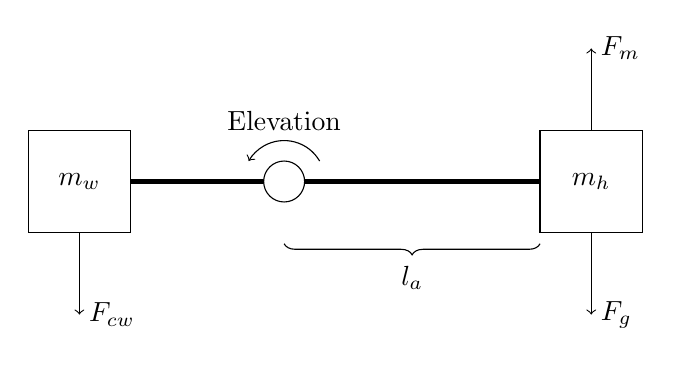
\begin{tikzpicture}[scale=1.3]
\usetikzlibrary{decorations.pathreplacing}
\path[draw,ultra thick] (1,1.5) -- (5,1.5);
\path[draw,fill=white] (0,1) rectangle ++(1,1) node[midway] {$m_w$};
\path[draw,fill=white] (5,1) rectangle ++(1,1) node[midway] {$m_h$};
\path[draw,fill=white] (2.5,1.5) circle (0.2);
\path[draw,->] (2.5,1.5) ++ (30:0.4) arc (30:150:0.4) node[midway, above] {Elevation};
\path[draw,->] (0.5,1) -- ++(0,-0.8) node[right] {$F_{cw}$};
\path[draw,->] (5.5,1) -- ++(0,-0.8) node[right] {$F_g$};
\path[draw,->] (5.5,2) -- ++(0,0.8) node[right] {$F_m$};
\path[draw,decorate,decoration={brace,amplitude=4pt,raise=4pt,mirror}] (2.5,1) -- (5,1)
node[midway, below=0.3cm] {$l_a$};
\end{tikzpicture}
    \caption{Helicopter body free body diagram.}
    \label{fig:heli_body_free_body}
\end{figure}\\
\begin{table}[tb]
	\centering
	\caption{Variables used in equations of motion.}
	\begin{tabular}{ll}
		\toprule
		Symbol & Variable \\
		\midrule
		$p$ & Pitch\\
		$p_c$ & Pitch reference\\
		$\lambda$ & Travel\\
		$r$ & Rate of travel\\
		$r_c$ & Rate of travel reference\\
		$e$ & Elevation\\
		$e_c$ & Elevation refernce\\
		$V_f$ & Voltage, front motor\\
		$V_b$ & Voltage, back motor\\
		$V_d$ & Voltage difference, $V_f - V_b$\\
		$V_s$ & Voltage sum, $V_f + V_b$\\
		$K_{pp},\,K_{pd},\,K_{ep},\,K_{ei},\,K_{ed}$ & Controller gains\\
		$T_g$ & Momentum needed to keep helicopter in air\\
		\bottomrule
	\end{tabular}
\label{tab:model_variables}
\end{table}